\chapter{Introduction} \label{chap:introduction} Since manufacturing processes involve the processes to transform raw materials into finished goods on a large scale, economists around the globe assert manufacturing to be a wealth-producing sector of an economy. Manufacturing world thrives upon many complex variables. In the recent years, due to innovations in Information and Communication Technology (\acs{ICT}) the focus of supply and demand are shifting, thus manufacturing industry is experiencing more complex supply chains. Customers demanding high levels of individualized products are driving fierce competition in pricing and forcing manufacturers to strive for highest levels of efficiencies. The kind of turbulences a manufacturer can expect now-a-days can be found in \reffig{fig:1.1}. Still manufacturers can develop effective survival strategies amidst all these turbulences, if they are able to continuously adapt their organizational structures \cite{WESTKAMP}.

The challenge lies in making the manufacturing adaptive by accessing all available information when it is needed, where it is needed, and in the form it is most useful to drive optimal actions and responses. Adaptive manufacturing also enables manufacturers to generate and apply data-driven manufacturing intelligence throughout the life-cycle of design, engineering, planning, and production.

\begin{figure}[h!]
	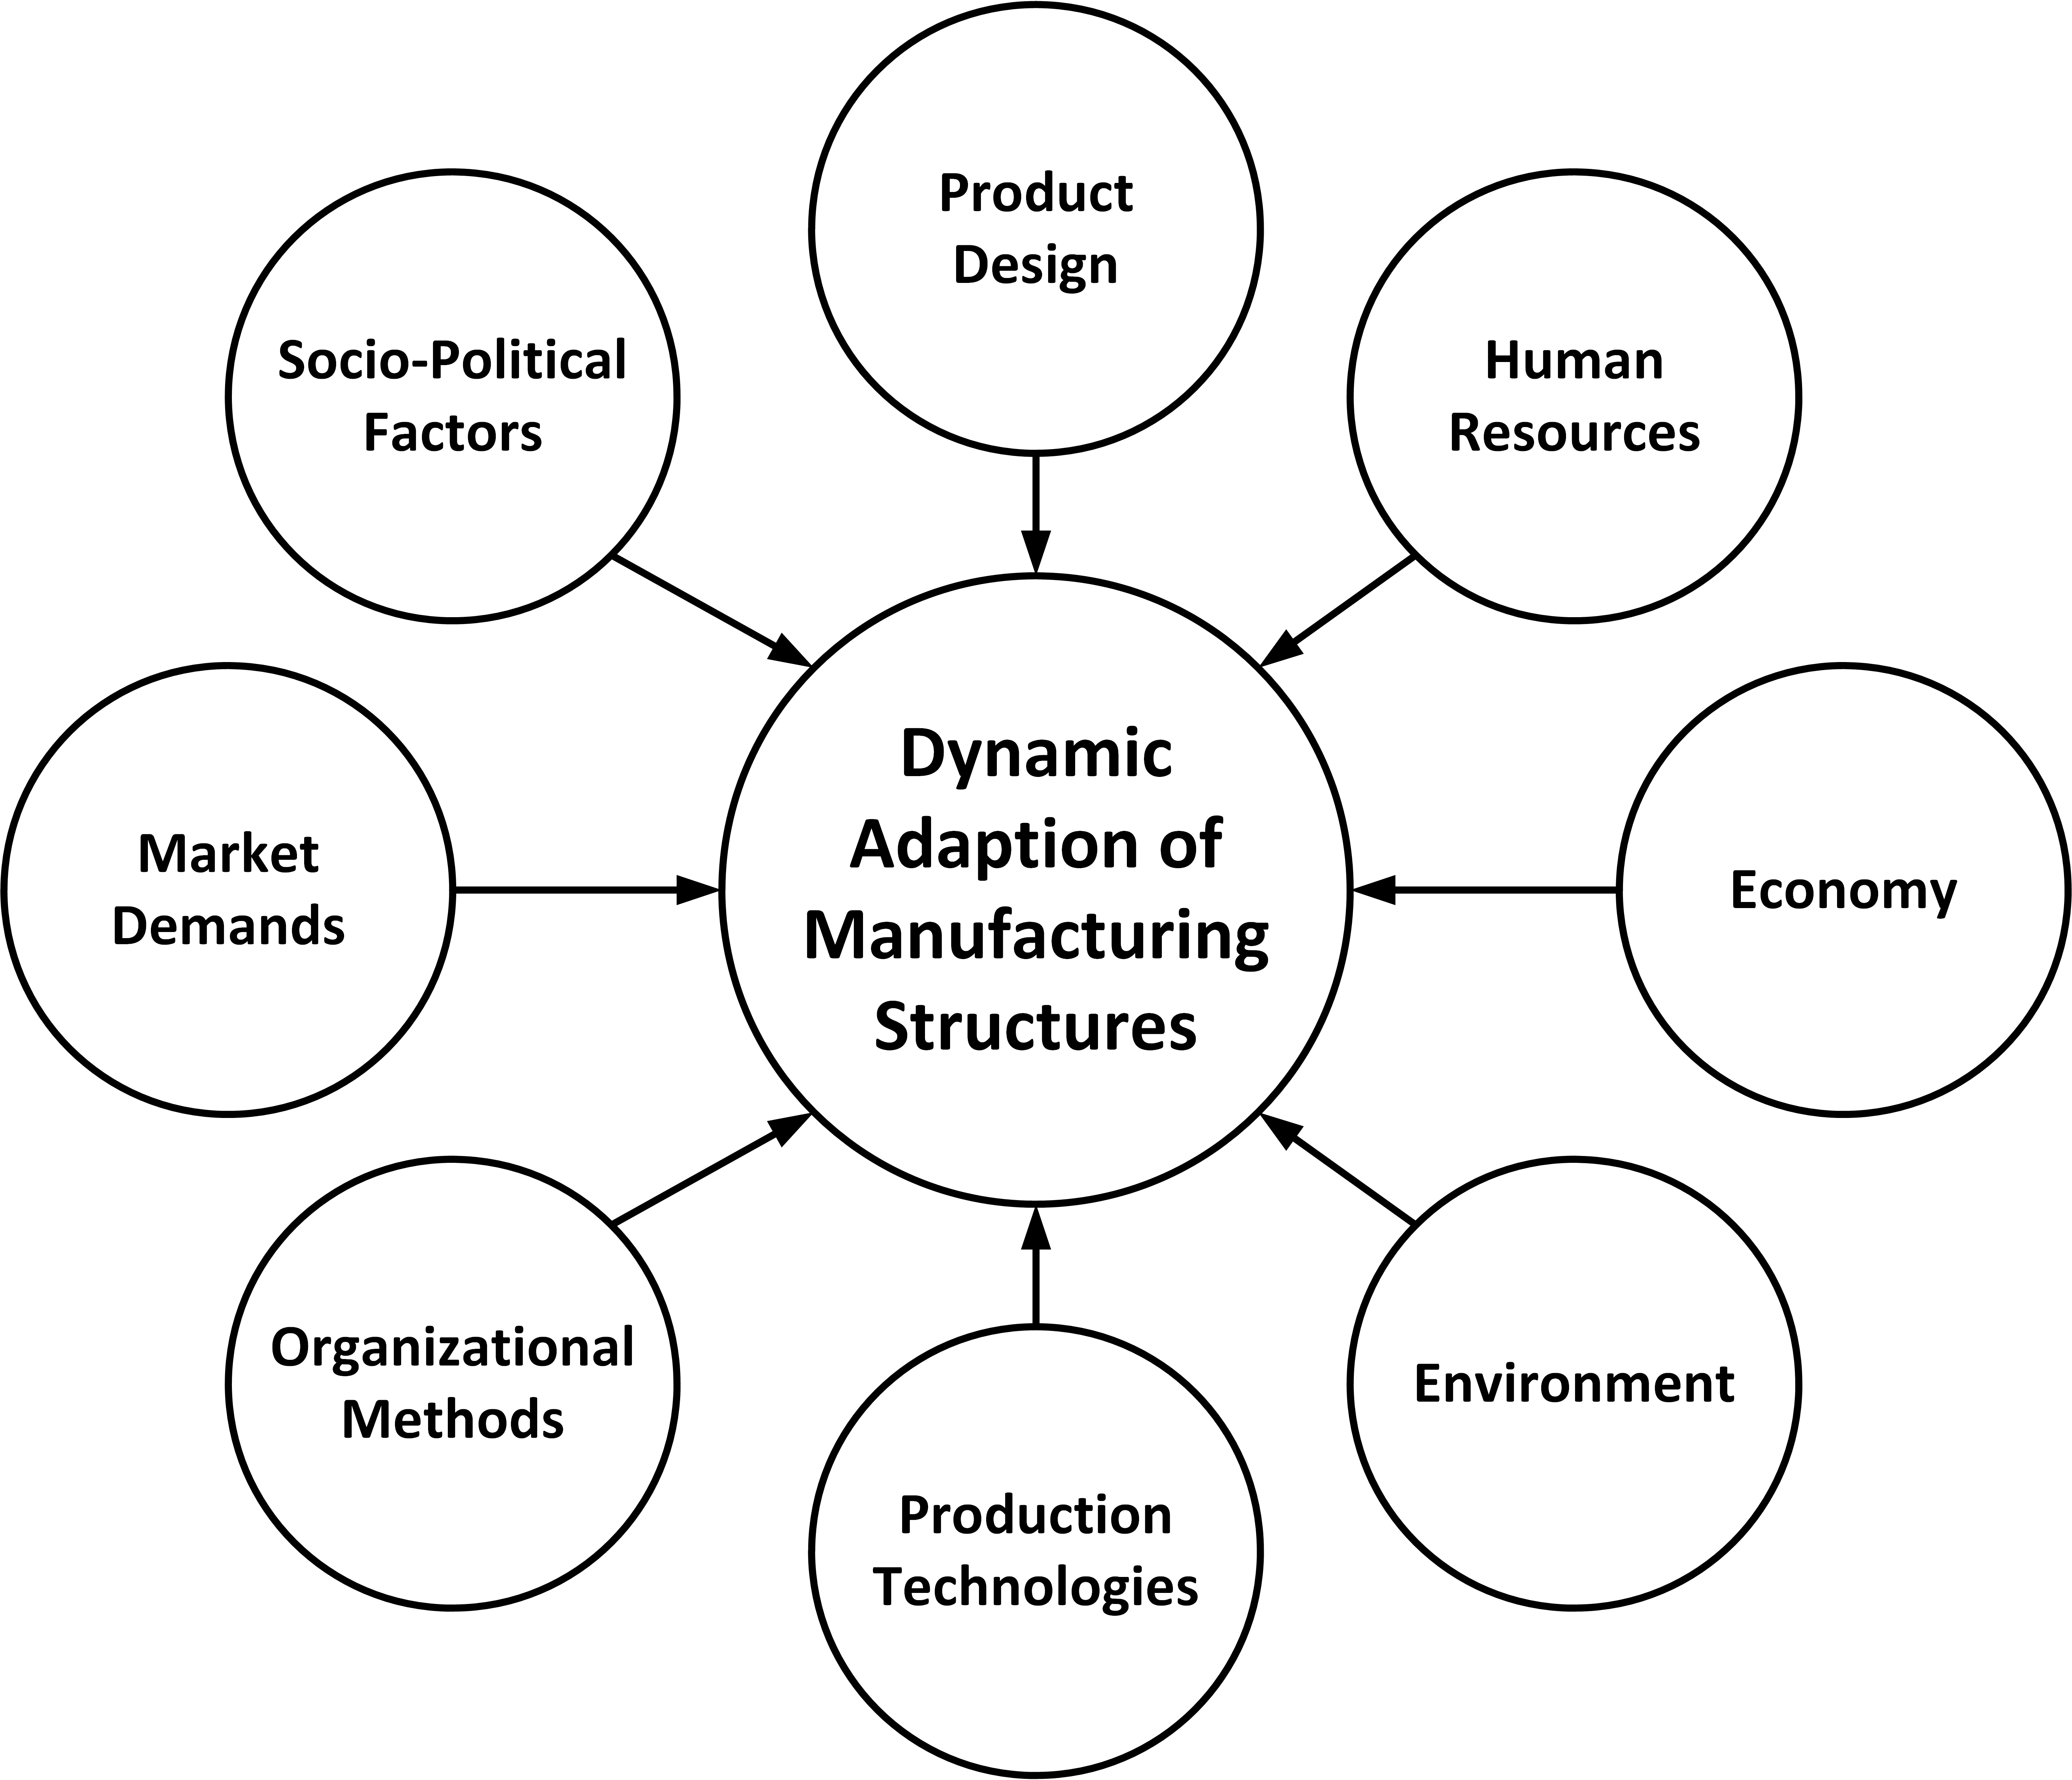
\includegraphics[scale=0.35]{./gfx/addmanustr}
	\centering
	\caption{Sources of Turbulences in Manufacturing - Adapted from \cite{WESTKAMP}}
	\label{fig:1.1}
\end{figure}

With the advent of a new wave of technological changes there is already driving a paradigm shift in manufacturing. Manufacturing sector is at the verge of a new industrial revolution which promises all range of opportunities for innovation in terms of smarter industrial processes, new business models and customized products. The new technological wave builds on the concept of interaction between the real and virtual worlds which becomes the core of the manufacturing processes. Both production equipment and manufactured products are now able to gather, process and analyze data of the physical world and interact with each other autonomously.

The primary objectives of production are known as the \textit{"Holy Trinity"} of cost, quality, and time. Some authors do refer this trio as \textit{"Iron Triangle"} \cite{BASUIRON}. Most important is to point out the right direction of goal achievement – low production costs, high quality of products, as well as short lead times in production and order processing. Recently the product variety on demand is added to these production goals. Products produced in series and not positioned within the lowest price segment can only be distinguished from competition by the ‘long tail’ of innumerable possible variants or individualized (customized) products - as we refer them \cite{LEANFAC}.

Erlach \cite{LEANFAC} explains the relationships between the four goal dimensions and the relevant goal conflicts by the logical square of goals shown in \reffig{fig:1.2}. In sum, the possible relationships between the four goal dimensions can be distinguished into following four types:
\begin{enumerate}
	\item The contradictory antagonism of goals describes the strongest type of conflict where goal achievement for the one goal deteriorates that of the other goal.
	\item The contrary antagonism of goals describes that the attainment of the two goals cannot be improved at the same time, though the fulfillment of the one goal can be improved without negatively affecting the fulfillment of the other goal.
	\item The subordination of goals is possible when attainment of some goals are basically easier to accomplish than others thanks to their lower implementable requirements.
	\item The compatibility of goals exists if the two goals can be better accomplished independently.
\end{enumerate}

Improving individual goals does not necessarily mean that another goal is affected to the same degree; some goals can actually be improved simultaneously. The objective of production optimization is to counterbalance operation of production and the product range at a specific production site with the four goal dimensions in order to achieve the best level of goal achievement \cite{LEANFAC}.

\begin{figure}[h!]
	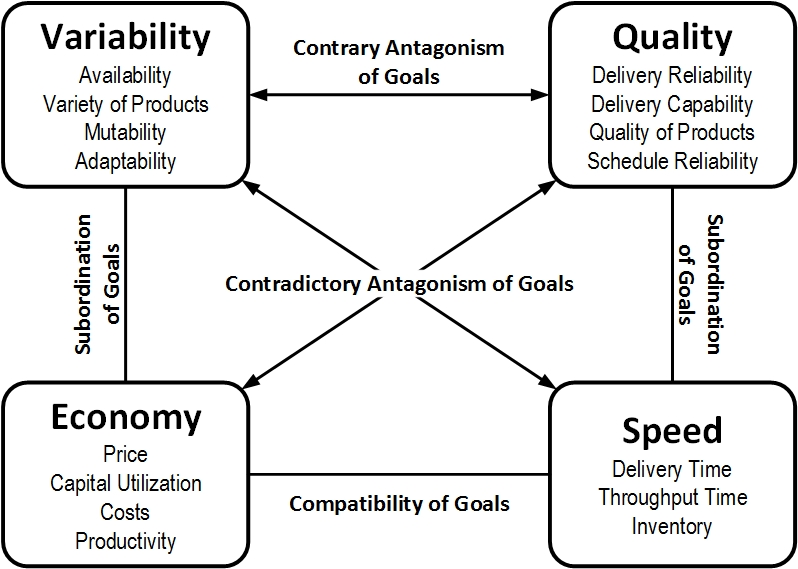
\includegraphics[scale=0.49]{./gfx/4goals}
	\centering
	\caption{Logical Four Square of Conflicting Goals of Production \cite{LEANFAC}}
	\label{fig:1.2}
\end{figure}

To increase the efficiency of production process, automation, optimization, and dynamic adaption became the most important requirements in manufacturing sector \cite{DBHENG}. Since the dawn of sensors and networking technologies, vital information can be gathered before-hand to decide the most suitable and optimized process. The selection of each execution step may depend on different factors as new technological advancements provide more solution options to the same kind of problems. Manually conducted assembly tasks may provide alternatives to the existing automation methods depending on the current demand, status of the machinery, and occupation of the machinery \cite{TIMURCIRP}. Situations can be observed using modern world smart-systems that enable the application of well-adopted business process modeling and execution  solutions in the context of manufacturing companies and tracking of activity flows in the real world \cite{CONWORKFLOW}.

To strengthen the case, a recent sector research work by Deutsche Bank \cite{DBHENG} can be looked upon. This predicts that Germany with its favorable fundamental features will find the next industrial revolution a major long-term opportunity to consolidate its leading position in the global marketplace even against its fast-growing emerging market competitors. Thus Germany has been and will remain an industrial heavyweight, creating one-third economy of the European Union (\acs{EU}) \cite{DBHENG}.

Production or Manufacturing processes can be modeled using business process modeling languages e.g. Business Process Execution Language (\acs{BPEL}) \cite{BPELSPEC} or Business Process Model and Notation (\acs{BPMN}) \cite{OMGSPEC}. After modeling, process models are deployed on compliant workflow engines for an automated execution. But these paradigms don't support adaptive and flexible execution of business processes in manufacturing sector. By not considering these adaptations, the manufacturing companies lose their revenue and edge in market by remaining reluctant to structural changes on time \cite{TIMURCIRP,CONWORKFLOW}.

\section{Problem Statement}
Manufacturing processes need to be updated regularly to stay competitive in the market. With the emergence of new sensor technologies, \textit{Internet of Things (\acs{IoT})} which is discussed later in \refsection{IOT}, the manufacturing processes can be made smarter to leverage the next industrial revolution - commonly referred as \textit{Industry 4.0}. We introduce Industry 4.0 in early part of the literature review in \refsection{ind4}.

Sungur et al. \cite{TIMURCIRP} presented a novel approach to support \textit{Context-sensitive Adaptive Production Process} in their research work. They extended production processes, which contain a sequence of predefined sets of sub-processes, with \textit{Context-sensitive Execution Steps (\acs{CES})}. For each \acs{CES}, context-relevant sub-processes are chosen and desired processes are elected, optimized, deployed and executed \cite{TIMURCIRP}. \acs{CES} approach dictates a way in which processes can possibly adapt themselves to the execution context. In each context, there can be multiple alternatives for the same process goals and the best needs to be selected and executed at runtime \cite{TIMURCIRP}. All details relevant to context-sensitive workflows have been discussed thoroughly later in \refsection{conces}.

In this thesis work, we define a \acs{BPMN} extension which do not change semantics of standard \acs{BPMN} if it's needed at all and adds the necessary details to make manufacturing process models executable. To create this extension, we have analyzed the properties that make \acs{CES}s unique and also scrutinized important and relevant \acs{BPMN} properties which might be vital during creation of the \acs{CES} extensions. These properties are later on used to derive our requirements from which we create our extension. A summary of the thesis work can be found below in \reffig{fig:1.3}.
\begin{figure}[h!]
	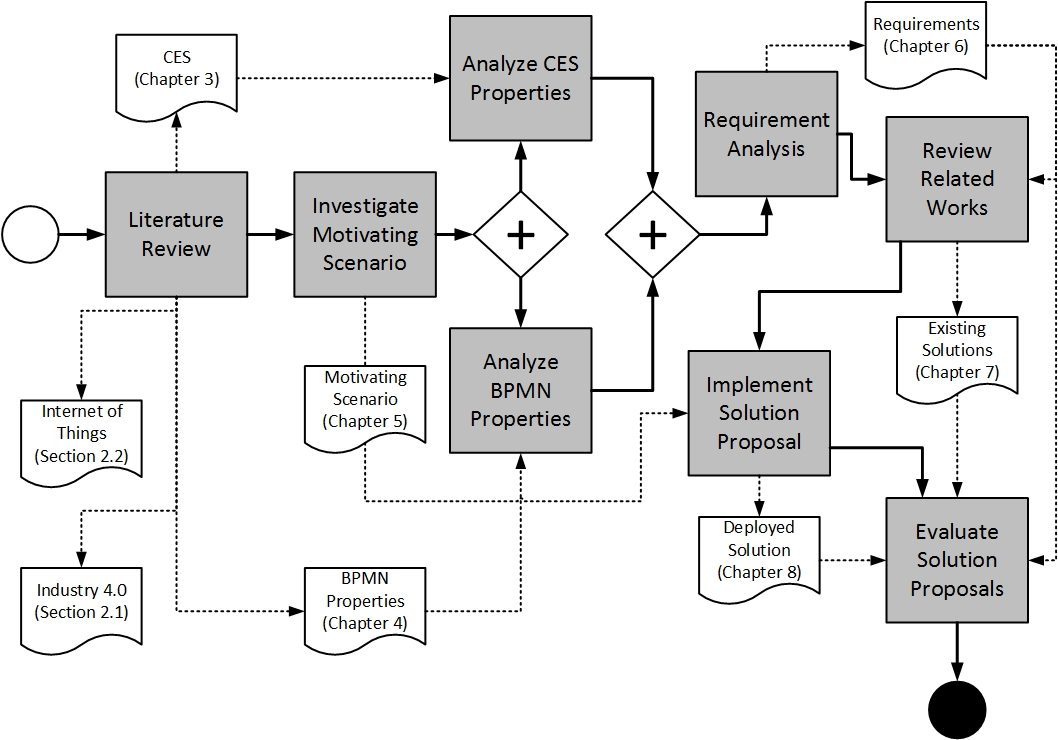
\includegraphics[scale=0.55]{./gfx/outline}
	\centering
	\caption{The Thesis Methodology Flow-chart - Inspired from \cite{TIMURTHESIS}}
	\label{fig:1.3}
\end{figure}
\section{Methodology and Outline}
The remaining thesis document is structured in the following way:
\begin{itemize}
	\item \textit{\refsection{chap:fundamentals} - Fundamentals:} The literature review of this thesis is carried out in three steps as suggested by Levy et al. \cite{LEVYLIT}. We analyze literature related with Industry 4.0 and Internet of Things ({\acs{IoT}}). Main focus during the literature review was to understand the current development in Industry 4.0 and it's implications in midst of the innovations in \acs{IoT} technologies. Trends in the \acs{IoT} field has also been discussed. 
	\item \textit{\refsection{conces} - Context-sensitive Workflows:} In the next chapter, we analyze literature related with Context-sensitive Execution Step (\acs{CES}). Properties and operational semantics of \acs{CES} are also discussed in the concluding section of the review. After necessary processing corresponding descriptions are touched upon in subsequent.
	\item \textit{\refsection{chap:bpmn} - Business Process Model and Notation:} The last part of the literature review is focused upon analyzing properties of \acs{CES} from the point of view of Business Process Management (\acs{BPM}), and the efficacies of \acs{BPMN}. This chapter has been added just before modeling the motivating scenario.
	\item \textit{\refsection{chap:motscene} - Motivating Scenario:} For the sake of analysis and apply the conceptual workflow modeling construct, we have described a motivating scenario depicting a real-world manufacturing scenario which is a mix of both manual- and automated tasks.
	\item \textit{\refsection{chap:requirements} - Requirement Analysis:} In this chapter, we derive our requirements from the properties that we have found related. By defining our requirements, we conclude the task requirement analysis in the methodology model \reffig{fig:1.3}. All the relevant properties and requirements for the \acs{CES} have been described in this chapter.
	\item \textit{\refsection{chap:relatedworks} - Related Works:} In the next task, we select and analyze few already existing extensions of \acs{BPMN} or any ongoing work in same direction. We propose our solution which satisfy the requirements that we have previously defined to make sure that our approach proposed by Sungur et al. \cite{TIMURCIRP} can cater the best to the manufacturing sector.
	\item \textit{\refsection{chap:archimpl} - Architecture and Implementation:} During the implementation of our conceptual construct, we use the \acs{BPMN} extension methodology and we preserve the semantics of the existing \acs{BPMN} properties. Architecture for the execution of modeled process is touched upon in this chapter.
	\item \textit{\refsection{chap:validationevaluation} - Evaluation:} 
	In our final task, we evaluate our approach by comparing it with the current state of art or related works already discussed in \refsection{chap:relatedworks}. We conclude this task by a thorough comparison between several existing solutions. 
	\item \textit{\refsection{chap:outcome} - Summary and Outlook:} 
	In the last chapter, we give a summary and an outlook about our contribution to the manufacturing world.
\end{itemize}

The thesis document also contains two appendices for the further look-up:
\begin{itemize}
	\item \textit{\refappendix{acronymlist} - List of Acronyms:} The list containing all the abbreviations or acronyms which are used in this document is added in this appendix.
	\item \textit{\refappendix{glossary} - Glossary:} This appendix is intended to define terms or concepts cited in the documented that are out of the scope of our discussion.
\end{itemize}
